% Options for packages loaded elsewhere
\PassOptionsToPackage{unicode}{hyperref}
\PassOptionsToPackage{hyphens}{url}
%
\documentclass[
]{article}
\usepackage{amsmath,amssymb}
\usepackage{iftex}
\ifPDFTeX
  \usepackage[T1]{fontenc}
  \usepackage[utf8]{inputenc}
  \usepackage{textcomp} % provide euro and other symbols
\else % if luatex or xetex
  \usepackage{unicode-math} % this also loads fontspec
  \defaultfontfeatures{Scale=MatchLowercase}
  \defaultfontfeatures[\rmfamily]{Ligatures=TeX,Scale=1}
\fi
\usepackage{lmodern}
\ifPDFTeX\else
  % xetex/luatex font selection
\fi
% Use upquote if available, for straight quotes in verbatim environments
\IfFileExists{upquote.sty}{\usepackage{upquote}}{}
\IfFileExists{microtype.sty}{% use microtype if available
  \usepackage[]{microtype}
  \UseMicrotypeSet[protrusion]{basicmath} % disable protrusion for tt fonts
}{}
\makeatletter
\@ifundefined{KOMAClassName}{% if non-KOMA class
  \IfFileExists{parskip.sty}{%
    \usepackage{parskip}
  }{% else
    \setlength{\parindent}{0pt}
    \setlength{\parskip}{6pt plus 2pt minus 1pt}}
}{% if KOMA class
  \KOMAoptions{parskip=half}}
\makeatother
\usepackage{xcolor}
\usepackage[margin=1in]{geometry}
\usepackage{color}
\usepackage{fancyvrb}
\newcommand{\VerbBar}{|}
\newcommand{\VERB}{\Verb[commandchars=\\\{\}]}
\DefineVerbatimEnvironment{Highlighting}{Verbatim}{commandchars=\\\{\}}
% Add ',fontsize=\small' for more characters per line
\usepackage{framed}
\definecolor{shadecolor}{RGB}{248,248,248}
\newenvironment{Shaded}{\begin{snugshade}}{\end{snugshade}}
\newcommand{\AlertTok}[1]{\textcolor[rgb]{0.94,0.16,0.16}{#1}}
\newcommand{\AnnotationTok}[1]{\textcolor[rgb]{0.56,0.35,0.01}{\textbf{\textit{#1}}}}
\newcommand{\AttributeTok}[1]{\textcolor[rgb]{0.13,0.29,0.53}{#1}}
\newcommand{\BaseNTok}[1]{\textcolor[rgb]{0.00,0.00,0.81}{#1}}
\newcommand{\BuiltInTok}[1]{#1}
\newcommand{\CharTok}[1]{\textcolor[rgb]{0.31,0.60,0.02}{#1}}
\newcommand{\CommentTok}[1]{\textcolor[rgb]{0.56,0.35,0.01}{\textit{#1}}}
\newcommand{\CommentVarTok}[1]{\textcolor[rgb]{0.56,0.35,0.01}{\textbf{\textit{#1}}}}
\newcommand{\ConstantTok}[1]{\textcolor[rgb]{0.56,0.35,0.01}{#1}}
\newcommand{\ControlFlowTok}[1]{\textcolor[rgb]{0.13,0.29,0.53}{\textbf{#1}}}
\newcommand{\DataTypeTok}[1]{\textcolor[rgb]{0.13,0.29,0.53}{#1}}
\newcommand{\DecValTok}[1]{\textcolor[rgb]{0.00,0.00,0.81}{#1}}
\newcommand{\DocumentationTok}[1]{\textcolor[rgb]{0.56,0.35,0.01}{\textbf{\textit{#1}}}}
\newcommand{\ErrorTok}[1]{\textcolor[rgb]{0.64,0.00,0.00}{\textbf{#1}}}
\newcommand{\ExtensionTok}[1]{#1}
\newcommand{\FloatTok}[1]{\textcolor[rgb]{0.00,0.00,0.81}{#1}}
\newcommand{\FunctionTok}[1]{\textcolor[rgb]{0.13,0.29,0.53}{\textbf{#1}}}
\newcommand{\ImportTok}[1]{#1}
\newcommand{\InformationTok}[1]{\textcolor[rgb]{0.56,0.35,0.01}{\textbf{\textit{#1}}}}
\newcommand{\KeywordTok}[1]{\textcolor[rgb]{0.13,0.29,0.53}{\textbf{#1}}}
\newcommand{\NormalTok}[1]{#1}
\newcommand{\OperatorTok}[1]{\textcolor[rgb]{0.81,0.36,0.00}{\textbf{#1}}}
\newcommand{\OtherTok}[1]{\textcolor[rgb]{0.56,0.35,0.01}{#1}}
\newcommand{\PreprocessorTok}[1]{\textcolor[rgb]{0.56,0.35,0.01}{\textit{#1}}}
\newcommand{\RegionMarkerTok}[1]{#1}
\newcommand{\SpecialCharTok}[1]{\textcolor[rgb]{0.81,0.36,0.00}{\textbf{#1}}}
\newcommand{\SpecialStringTok}[1]{\textcolor[rgb]{0.31,0.60,0.02}{#1}}
\newcommand{\StringTok}[1]{\textcolor[rgb]{0.31,0.60,0.02}{#1}}
\newcommand{\VariableTok}[1]{\textcolor[rgb]{0.00,0.00,0.00}{#1}}
\newcommand{\VerbatimStringTok}[1]{\textcolor[rgb]{0.31,0.60,0.02}{#1}}
\newcommand{\WarningTok}[1]{\textcolor[rgb]{0.56,0.35,0.01}{\textbf{\textit{#1}}}}
\usepackage{graphicx}
\makeatletter
\def\maxwidth{\ifdim\Gin@nat@width>\linewidth\linewidth\else\Gin@nat@width\fi}
\def\maxheight{\ifdim\Gin@nat@height>\textheight\textheight\else\Gin@nat@height\fi}
\makeatother
% Scale images if necessary, so that they will not overflow the page
% margins by default, and it is still possible to overwrite the defaults
% using explicit options in \includegraphics[width, height, ...]{}
\setkeys{Gin}{width=\maxwidth,height=\maxheight,keepaspectratio}
% Set default figure placement to htbp
\makeatletter
\def\fps@figure{htbp}
\makeatother
\setlength{\emergencystretch}{3em} % prevent overfull lines
\providecommand{\tightlist}{%
  \setlength{\itemsep}{0pt}\setlength{\parskip}{0pt}}
\setcounter{secnumdepth}{-\maxdimen} % remove section numbering
\ifLuaTeX
  \usepackage{selnolig}  % disable illegal ligatures
\fi
\usepackage{bookmark}
\IfFileExists{xurl.sty}{\usepackage{xurl}}{} % add URL line breaks if available
\urlstyle{same}
\hypersetup{
  pdftitle={Skincare Write-Up},
  pdfauthor={Sofia Ward / Bowie Chuang / Christina Pham / Carter Kulm},
  hidelinks,
  pdfcreator={LaTeX via pandoc}}

\title{Skincare Write-Up}
\author{Sofia Ward / Bowie Chuang / Christina Pham / Carter Kulm}
\date{2025-03-11}

\begin{document}
\maketitle

\section{Curated Sephora Skincare Generator
3000000}\label{curated-sephora-skincare-generator-3000000}

\subsection{Content Based Filtering Recommendation
System}\label{content-based-filtering-recommendation-system}

\begin{center}\rule{0.5\linewidth}{0.5pt}\end{center}

\section{Introduction}\label{introduction}

With the growing number of skincare products available, choosing the
right one for an individual's specific needs can be overwhelming. To
help users navigate this vast selection, we developed a content-based
skincare recommendation system that suggests products based on their
attributes and similarity to other items.

We wanted to build something that would save users money and time from
trying product after product, since everyone's skin is different!
Advertising and reviews are misleading since company goals don't align
with the user's best interest: finding the right skincare! Our model not
only selects products based on similarity, but also incorporates
ingredient lists, skin types, and targeted skin concerns. This filtering
gives users 10 individually catered products to their specific needs.
For user accessibility we chose Sephora's Skincare selection.

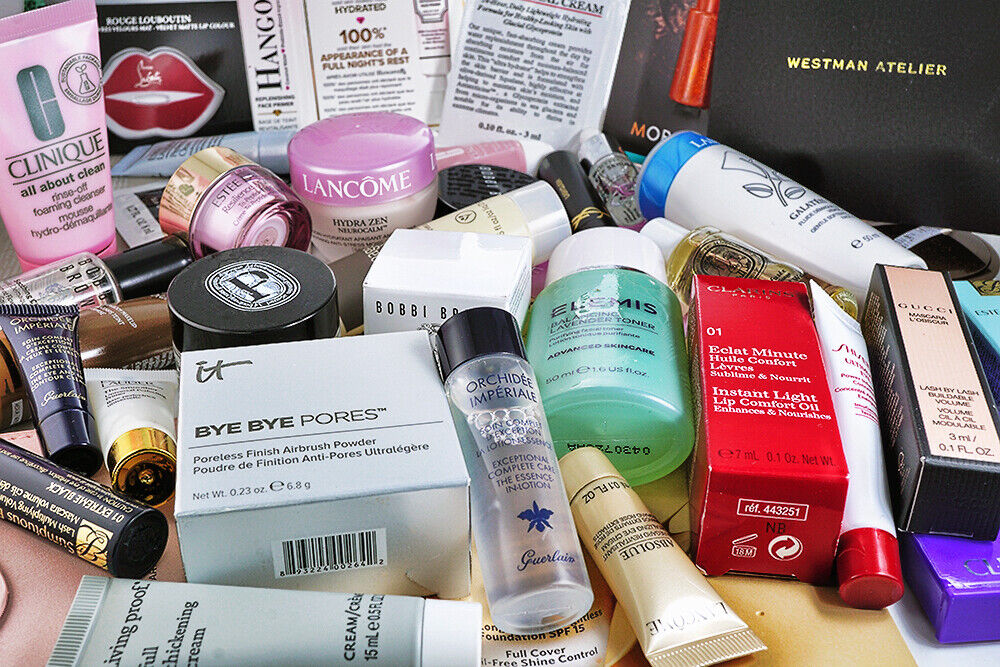
\includegraphics[width=4.1875in,height=\textheight]{data/s-l1200.jpg}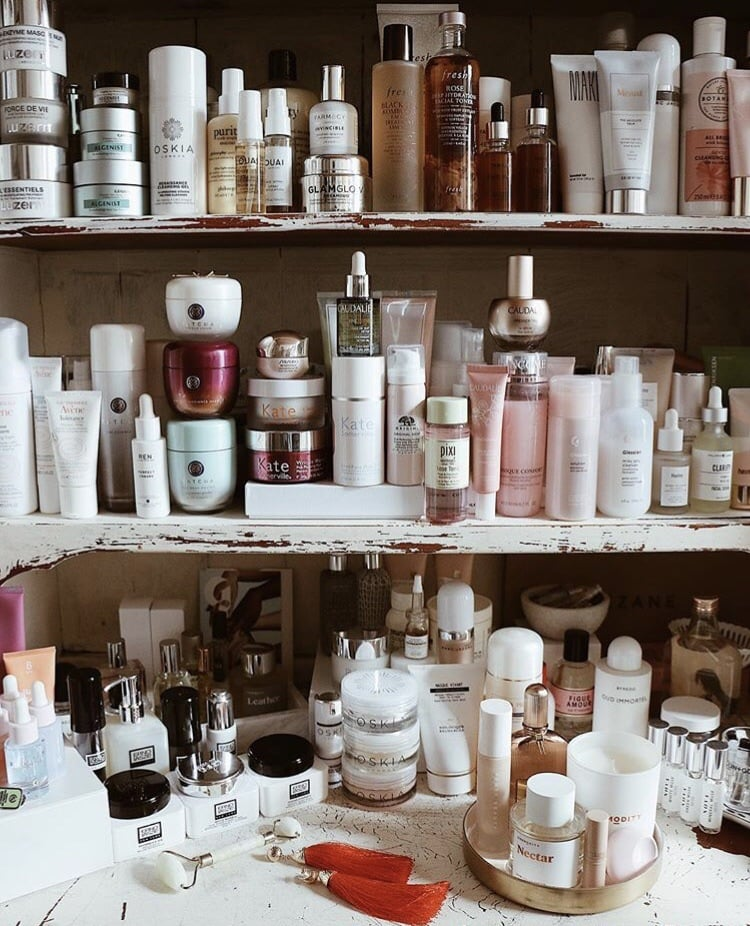
\includegraphics[width=2.26042in,height=\textheight]{data/prod.jpeg}

\subsubsection{Web-scraped Data
Description}\label{web-scraped-data-description}

To build our skincare recommendation system, we collected product data
from the Sephora website using web scraping techniques. After checking
for permissions, we used the robots.txt file to acquire an html of
\href{https://www.sephora.com/sitemaps/products-sitemap_en-CA.xml}{product
links}, utilizing Selenium's Webdriver and Beautiful Soup. Filtering
cosmetics and hair products left us with a categorized link data frame
to begin web-scraping!

We encountered several obstacles but through trial and error extracted
our information; pop-up ads, scroll-down functionality, custom
user-agent strings to avoid bot detection. Scraping itself took copious
amounts of time, and we found that smaller segments extracted less
N/A's. Altogether we scraped \textbf{1,888 links} which filtered out to
\textbf{800 observations and 12 columns.} The final scraping loop is
provided in the appendix of this report.

\begin{verbatim}
## [1] "Dimensions:  799" "Dimensions:  12"
\end{verbatim}

The data set contains key attributes essential for content-based
filtering, including:

\begin{itemize}
\tightlist
\item
  \textbf{Product Name}: The name of the skincare product.
\item
  \textbf{Brand}: The company or brand that manufactures the product.
\item
  \textbf{Category}: The type of product: exfoliates, cleansers, toners,
  serums, moisturizer, masks).
\item
  \textbf{Price}: The cost of the product in USD.
\item
  \textbf{Reviews}: The number of user reviews for the product.
\item
  \textbf{Size}: The quantity of the product (e.g., 100ml, 1.7oz).
\item
  \textbf{Ingredients}: A list of active and inactive ingredients.
\item
  \textbf{Description}: A textual summary of the product, often provided
  by the brand or Sephora.
\item
  \textbf{Skin Concern}: The specific skin issues the product addresses
  (e.g., acne, dryness, hyper-pigmentation).
\item
  \textbf{Skin Type}: The recommended skin types for the product (e.g.,
  oily, dry, combination).
\end{itemize}

\begin{center}\rule{0.5\linewidth}{0.5pt}\end{center}

\section{Methodology}\label{methodology}

\subsection{Data Pre-processing}\label{data-pre-processing}

After collecting the raw data, we performed several pre-processing
steps:

\begin{enumerate}
\def\labelenumi{\arabic{enumi}.}
\item
  \textbf{Cleaning the Data}: Removed duplicate entries and handled
  missing values through imputation or deletion.
\item
  \textbf{Feature Engineering}: Formatted price, rating, and size for
  consistency.
\end{enumerate}

\begin{Shaded}
\begin{Highlighting}[]
\NormalTok{filter }\OtherTok{\textless{}{-}}\NormalTok{ filter }\SpecialCharTok{\%\textgreater{}\%} 
  \FunctionTok{mutate}\NormalTok{(}\FunctionTok{across}\NormalTok{(}\StringTok{\textasciigrave{}}\AttributeTok{Product Price}\StringTok{\textasciigrave{}}\NormalTok{, }\SpecialCharTok{\textasciitilde{}} \FunctionTok{as.numeric}\NormalTok{(}\FunctionTok{gsub}\NormalTok{(}\StringTok{"}\SpecialCharTok{\textbackslash{}\textbackslash{}}\StringTok{$"}\NormalTok{, }\StringTok{""}\NormalTok{, .)))) }\SpecialCharTok{\%\textgreater{}\%}  \CommentTok{\# take $ out of price}
  \FunctionTok{mutate}\NormalTok{(}
    \StringTok{\textasciigrave{}}\AttributeTok{Product Price}\StringTok{\textasciigrave{}} \OtherTok{=} \FunctionTok{as.numeric}\NormalTok{(}\StringTok{\textasciigrave{}}\AttributeTok{Product Price}\StringTok{\textasciigrave{}}\NormalTok{),      }\CommentTok{\# Ensure numeric conversions}
    \StringTok{\textasciigrave{}}\AttributeTok{Product Rating}\StringTok{\textasciigrave{}} \OtherTok{=} \FunctionTok{round}\NormalTok{(}\FunctionTok{as.numeric}\NormalTok{(}\StringTok{\textasciigrave{}}\AttributeTok{Product Rating}\StringTok{\textasciigrave{}}\NormalTok{), }\DecValTok{1}\NormalTok{), }
    \StringTok{\textasciigrave{}}\AttributeTok{Product Reviews}\StringTok{\textasciigrave{}} \OtherTok{=} \FunctionTok{as.numeric}\NormalTok{(}\StringTok{\textasciigrave{}}\AttributeTok{Product Reviews}\StringTok{\textasciigrave{}}\NormalTok{)) }\SpecialCharTok{\%\textgreater{}\%} 
  \FunctionTok{mutate}\NormalTok{(}\StringTok{\textasciigrave{}}\AttributeTok{Product Size}\StringTok{\textasciigrave{}} \OtherTok{=} \FunctionTok{case\_when}\NormalTok{( }
      \StringTok{\textasciigrave{}}\AttributeTok{Product Size}\StringTok{\textasciigrave{}} \SpecialCharTok{==} \StringTok{"N/A"} \SpecialCharTok{\textasciitilde{}} \StringTok{"No Size"}\NormalTok{, }
      \ConstantTok{TRUE} \SpecialCharTok{\textasciitilde{}} \StringTok{\textasciigrave{}}\AttributeTok{Product Size}\StringTok{\textasciigrave{}}      \CommentTok{\# change N/A to No size}
\NormalTok{    ) )}

\NormalTok{filter }\SpecialCharTok{\%\textgreater{}\%} 
  \FunctionTok{select}\NormalTok{(}\StringTok{\textasciigrave{}}\AttributeTok{Product Price}\StringTok{\textasciigrave{}}\NormalTok{, }\StringTok{\textasciigrave{}}\AttributeTok{Product Rating}\StringTok{\textasciigrave{}}\NormalTok{, }\StringTok{\textasciigrave{}}\AttributeTok{Product Reviews}\StringTok{\textasciigrave{}}\NormalTok{) }\SpecialCharTok{\%\textgreater{}\%} 
  \FunctionTok{head}\NormalTok{()}
\end{Highlighting}
\end{Shaded}

\begin{verbatim}
## # A tibble: 6 x 3
##   `Product Price` `Product Rating` `Product Reviews`
##             <dbl>            <dbl>             <dbl>
## 1             108              4.1                74
## 2              26              4.6               269
## 3              39              4.3               486
## 4              52              4.4                58
## 5              18              4.6               498
## 6               7              4.3               448
\end{verbatim}

\subsection{Recommendation System: Content-Based
Filtering}\label{recommendation-system-content-based-filtering}

Our system uses \textbf{content-based filtering}, a recommendation
approach that suggests products based on their attributes rather than
user interactions. We opted for this approach to respect the privacy of
Sephora's customers and for user accessibility.

\subsubsection{\texorpdfstring{\textbf{What is Content-Based
Filtering?}}{What is Content-Based Filtering?}}\label{what-is-content-based-filtering}

Content-based filtering analyzes the characteristics of items to
recommend similar products. Instead of relying on user behavior (as in
collaborative filtering), it compares the features of a given product to
those of other products in the data set. In our project, we used cosine
similarity and the sigmoid kernel to generate personalized product
recommendations which allows us to explore how different similarity
metrics impact recommendation results.

\subsubsection{Cosine Similarity Content-Based Recommender
System}\label{cosine-similarity-content-based-recommender-system}

For the \emph{cosine similarity} based recommender system, we represent
each skincare product as a \textbf{feature vector}, incorporating
product descriptions, ingredients, category, skin concerns, and other
relevant attributes. The similarity between products is calculated using
\textbf{cosine similarity}, which measures the angle between two vectors
in a multidimensional space. A higher cosine similarity score indicates
that two products are more alike.

Mathematically, cosine similarity between two product vectors \textbf{A}
and \textbf{B} is given by:

\[
S_C(A, B) = \cos(\theta) = \frac{A \cdot B}{\|A\| \|B\|}
\]

Where:

\begin{itemize}
\tightlist
\item
  \(A \cdot B\) is the dot product of the two vectors,
\item
  \(\|A\|\) and \(\|B\|\) are the magnitudes of the vectors.
\end{itemize}

Using this approach, when a user selects a product, the system finds
other products with the highest cosine similarity, ensuring
recommendations are tailored to the product's attributes!

\subsection{Implementation}\label{implementation}

We implemented the recommendation system in \textbf{Python}, using
\texttt{scikit-learn} for text vectorization and similarity
computations. The key steps include:

\begin{enumerate}
\def\labelenumi{\arabic{enumi}.}
\tightlist
\item
  \textbf{Text Vectorization}: We converted textual data (e.g.,
  ingredients, descriptions) into vectors using \textbf{TF-IDF (Term
  Frequency-Inverse Document Frequency)}.
\end{enumerate}

\begin{verbatim}
## <Compressed Sparse Row sparse matrix of dtype 'float64'
##  with 94868 stored elements and shape (785, 7249)>
\end{verbatim}

\begin{enumerate}
\def\labelenumi{\arabic{enumi}.}
\setcounter{enumi}{1}
\tightlist
\item
  \textbf{Similarity Calculation}: We computed pairwise cosine
  similarity scores between products.
\end{enumerate}

\begin{Shaded}
\begin{Highlighting}[]
\NormalTok{cosine\_similarity }\OperatorTok{=}\NormalTok{ cosine\_similarity(tfidf\_matrix)}

\NormalTok{similarity\_df }\OperatorTok{=}\NormalTok{ pd.DataFrame(cosine\_similarity, }
\NormalTok{                index }\OperatorTok{=}\NormalTok{ df\_recommend2[}\StringTok{\textquotesingle{}Product Name\textquotesingle{}}\NormalTok{], }
\NormalTok{                columns }\OperatorTok{=}\NormalTok{ df\_recommend2[}\StringTok{\textquotesingle{}Product Name\textquotesingle{}}\NormalTok{]}
\NormalTok{                )}

\NormalTok{similarity\_df.head()}
\end{Highlighting}
\end{Shaded}

\begin{verbatim}
## Product Name                                        Cleanser  ...  Hydrating Hand Mask in Coconut + Mango
## Product Name                                                  ...                                        
## Cleanser                                            1.000000  ...                                0.052619
## Aquarius BHA + Blue Tansy Clarifying Cleanser       0.186218  ...                                0.073342
## Alpha Beta® AHA/BHA Daily Cleansing Gel             0.196730  ...                                0.062815
## Equilibrium™ Rebalancing Cream Cleanser             0.118336  ...                                0.048804
## Mini The POREfessional Get Unblocked Makeup-Rem...  0.097199  ...                                0.111556
## 
## [5 rows x 785 columns]
\end{verbatim}

\begin{enumerate}
\def\labelenumi{\arabic{enumi}.}
\setcounter{enumi}{2}
\tightlist
\item
  \textbf{Recommendation Generation}: For a given product, the system
  returns the top \textbf{10} most recommended products based on
  similarity scores.
\end{enumerate}

\begin{Shaded}
\begin{Highlighting}[]
\KeywordTok{def}\NormalTok{ give\_recommendation(product\_name):}
\NormalTok{    product\_index }\OperatorTok{=}\NormalTok{ similarity\_df.index.get\_loc(product\_name)}
\NormalTok{    top\_10 }\OperatorTok{=}\NormalTok{ similarity\_df.iloc[product\_index].sort\_values(ascending}\OperatorTok{=}\VariableTok{False}\NormalTok{)[}\DecValTok{1}\NormalTok{:}\DecValTok{11}\NormalTok{].reset\_index()}
\NormalTok{    top\_10.columns }\OperatorTok{=}\NormalTok{ [}\StringTok{\textquotesingle{}Product Name\textquotesingle{}}\NormalTok{, }\StringTok{"Similarity Rating"}\NormalTok{]}
\NormalTok{    top10\_product\_values }\OperatorTok{=}\NormalTok{ pd.Series(top\_10.index, index }\OperatorTok{=}\NormalTok{ top\_10[}\StringTok{\textquotesingle{}Product Name\textquotesingle{}}\NormalTok{])}
\NormalTok{    top\_10[}\StringTok{\textquotesingle{}Product Rating\textquotesingle{}}\NormalTok{] }\OperatorTok{=}\NormalTok{ df\_recommend2[}\StringTok{"Product Rating"}\NormalTok{].iloc[top10\_product\_values].values}
    \BuiltInTok{print}\NormalTok{(}\SpecialStringTok{f"Recommendations for customers buying }\SpecialCharTok{\{}\NormalTok{product\_name}\SpecialCharTok{\}}\SpecialStringTok{ :}\CharTok{\textbackslash{}n}\SpecialStringTok{"}\NormalTok{)}
    \ControlFlowTok{return}\NormalTok{ top\_10.style.set\_properties(}\OperatorTok{**}\NormalTok{\{}\StringTok{"background{-}color"}\NormalTok{: }\StringTok{"white"}\NormalTok{,}\StringTok{"color"}\NormalTok{:}\StringTok{"black"}\NormalTok{,}\StringTok{"border"}\NormalTok{: }\StringTok{"1.5px solid black"}\NormalTok{\})}
  
\NormalTok{give\_recommendation(}\StringTok{"Vinoclean Gentle Cleansing Almond Milk"}\NormalTok{)}
\end{Highlighting}
\end{Shaded}

\subsubsection{Sigmoid Kernel Content-Based Recommender
System}\label{sigmoid-kernel-content-based-recommender-system}

Next, we implemented another recommender system using the \emph{sigmoid
kernel}. This method transforms the similarity computation through a
nonlinear function, allowing it to detect nuanced connections that may
not be captured by linear measures like cosine similarity.

\[S_K(x, B) = \tanh(\alpha (x^T \cdot B) + c)\] - x: the feature vector
representing the input product - tanh: The hyperbolic tangent function.
- α: A scaling parameter that adjusts how sensitive the kernel is to the
similarity score. - xᵀ: the transpose of the feature vector representing
the input product. - B: the feature vector of another product in the
dataset that we want to compare with x. - xᵀ · y: the dot product
between the two vectors. - c: a bias term that shifts the output of the
kernel function.

\begin{enumerate}
\def\labelenumi{\arabic{enumi}.}
\item
  \textbf{Text Vectorization}: We use the same text vectorization as our
  cosine similarity recommender system.
\item
  \textbf{Similarity Calculation}: We compute the pairwise similarities
  between all items in the tfv\_matrix, resulting in a similarity matrix
  called sig (denoted as S). This is a square matrix where both the rows
  and columns correspond to items---in this case, product names---and
  each cell (i,𝑗)represents the similarity score between item i and item
  j based on the sigmoid kernel. To facilitate lookup, we use the
  Series() function to map product names to their corresponding indices.
\end{enumerate}

\begin{Shaded}
\begin{Highlighting}[]
\ImportTok{import}\NormalTok{ pandas }\ImportTok{as}\NormalTok{ pd}
\ImportTok{import}\NormalTok{ numpy }\ImportTok{as}\NormalTok{ np}
\ImportTok{from}\NormalTok{ sklearn.feature\_extraction.text }\ImportTok{import}\NormalTok{ TfidfVectorizer}
\ImportTok{from}\NormalTok{ sklearn.metrics.pairwise }\ImportTok{import}\NormalTok{ sigmoid\_kernel}
\ImportTok{import}\NormalTok{ openpyxl}
\ImportTok{import}\NormalTok{ string}

\NormalTok{sig }\OperatorTok{=}\NormalTok{ sigmoid\_kernel(tfidf\_matrix, tfidf\_matrix)}
\NormalTok{df\_index }\OperatorTok{=}\NormalTok{ pd.Series(df\_recommend2.index, index }\OperatorTok{=}\NormalTok{ df\_recommend2[}\StringTok{\textquotesingle{}Product Name\textquotesingle{}}\NormalTok{])}
\KeywordTok{def}\NormalTok{ give\_recommendation2(product\_name, sig }\OperatorTok{=}\NormalTok{ sig):}
\NormalTok{    idx }\OperatorTok{=}\NormalTok{ df\_index[product\_name]}
\NormalTok{    sig\_score }\OperatorTok{=} \BuiltInTok{list}\NormalTok{(}\BuiltInTok{enumerate}\NormalTok{(sig[idx]))}
\NormalTok{    sig\_score }\OperatorTok{=} \BuiltInTok{sorted}\NormalTok{(sig\_score, key }\OperatorTok{=} \KeywordTok{lambda}\NormalTok{ x: x[}\DecValTok{1}\NormalTok{], reverse }\OperatorTok{=} \VariableTok{True}\NormalTok{)}\CommentTok{\# start at 1 to avoid the diagonal/same comparison}
\NormalTok{    sig\_score }\OperatorTok{=}\NormalTok{ sig\_score[}\DecValTok{1}\NormalTok{:}\DecValTok{11}\NormalTok{]}
\NormalTok{    product\_indices }\OperatorTok{=}\NormalTok{ [i[}\DecValTok{0}\NormalTok{] }\ControlFlowTok{for}\NormalTok{ i }\KeywordTok{in}\NormalTok{ sig\_score]}
    
\NormalTok{    rec\_dic }\OperatorTok{=}\NormalTok{ \{}\StringTok{"No"}\NormalTok{ : }\BuiltInTok{range}\NormalTok{(}\DecValTok{1}\NormalTok{,}\DecValTok{11}\NormalTok{), }
               \StringTok{"Product Name"}\NormalTok{ : df\_recommend2[}\StringTok{"Product Name"}\NormalTok{].iloc[product\_indices].values, }
               \StringTok{"Product Rating"}\NormalTok{: df\_recommend2[}\StringTok{"Product Rating"}\NormalTok{].iloc[product\_indices].values\}}
\NormalTok{    dataframe }\OperatorTok{=}\NormalTok{ pd.DataFrame(data }\OperatorTok{=}\NormalTok{ rec\_dic)}
\NormalTok{    dataframe.set\_index(}\StringTok{"No"}\NormalTok{, inplace }\OperatorTok{=} \VariableTok{True}\NormalTok{)}
\NormalTok{    dataframe[}\StringTok{\textquotesingle{}Product Rating\textquotesingle{}}\NormalTok{] }\OperatorTok{=}\NormalTok{ dataframe[}\StringTok{\textquotesingle{}Product Rating\textquotesingle{}}\NormalTok{].}\BuiltInTok{round}\NormalTok{(}\DecValTok{2}\NormalTok{)}
    
    \BuiltInTok{print}\NormalTok{(}\SpecialStringTok{f"Skin Care Recommendations for customers buying }\SpecialCharTok{\{}\NormalTok{product\_name}\SpecialCharTok{\}}\SpecialStringTok{ :}\CharTok{\textbackslash{}n}\SpecialStringTok{"}\NormalTok{)}
    \ControlFlowTok{return}\NormalTok{ dataframe.style.set\_properties(}\OperatorTok{**}\NormalTok{\{}\StringTok{"background{-}color"}\NormalTok{: }\StringTok{"white"}\NormalTok{,}\StringTok{"color"}\NormalTok{:}\StringTok{"black"}\NormalTok{,}\StringTok{"border"}\NormalTok{: }\StringTok{"1.5px  solid black"}\NormalTok{\})}
\end{Highlighting}
\end{Shaded}

\begin{enumerate}
\def\labelenumi{\arabic{enumi}.}
\setcounter{enumi}{2}
\tightlist
\item
  \textbf{Recommendation Generation}: Similarly, for any given product,
  the system returns the top \textbf{10} most recommended products based
  on similarity scores.
\end{enumerate}

\begin{Shaded}
\begin{Highlighting}[]
\NormalTok{give\_recommendation2(}\StringTok{"Vinoclean Gentle Cleansing Almond Milk"}\NormalTok{)}
\end{Highlighting}
\end{Shaded}

\begin{center}\rule{0.5\linewidth}{0.5pt}\end{center}

\section{EDA Visuals}\label{eda-visuals}

To better understand the composition and characteristics of the skincare
product dataset, we visualized key variables such as product category,
rating, price, and number of reviews.

\subsubsection{Distribution of Product
Category}\label{distribution-of-product-category}

We begin by examining how the products are distributed across different
categories. This helps us identify which types of skincare products are
most represented in the dataset.

\begin{Shaded}
\begin{Highlighting}[]
\NormalTok{filter }\SpecialCharTok{\%\textgreater{}\%}
  \FunctionTok{group\_by}\NormalTok{(}\StringTok{\textasciigrave{}}\AttributeTok{Product Category}\StringTok{\textasciigrave{}}\NormalTok{) }\SpecialCharTok{\%\textgreater{}\%}
  \FunctionTok{summarise}\NormalTok{(}\AttributeTok{Product\_Type =} \FunctionTok{n}\NormalTok{()) }\SpecialCharTok{\%\textgreater{}\%}
  \FunctionTok{ggplot}\NormalTok{(}\FunctionTok{aes}\NormalTok{(}\AttributeTok{x =} \FunctionTok{reorder}\NormalTok{(}\StringTok{\textasciigrave{}}\AttributeTok{Product Category}\StringTok{\textasciigrave{}}\NormalTok{, }\SpecialCharTok{{-}}\NormalTok{Product\_Type), }\AttributeTok{y =}\NormalTok{ Product\_Type, }\AttributeTok{fill =} \StringTok{\textasciigrave{}}\AttributeTok{Product Category}\StringTok{\textasciigrave{}}\NormalTok{)) }\SpecialCharTok{+}
  \FunctionTok{geom\_col}\NormalTok{() }\SpecialCharTok{+}
  \FunctionTok{labs}\NormalTok{(}
    \AttributeTok{title =} \StringTok{"Distribution of Product Types"}\NormalTok{,}
    \AttributeTok{x =} \StringTok{"Product Category"}\NormalTok{,}
    \AttributeTok{y =} \StringTok{"Number of Products"}
\NormalTok{  ) }\SpecialCharTok{+}
  \FunctionTok{theme\_minimal}\NormalTok{() }\SpecialCharTok{+}
  \FunctionTok{scale\_fill\_brewer}\NormalTok{(}\AttributeTok{palette =} \StringTok{"Set2"}\NormalTok{) }\SpecialCharTok{+} 
  \FunctionTok{coord\_flip}\NormalTok{() }\SpecialCharTok{+}  
  \FunctionTok{theme}\NormalTok{(}\AttributeTok{plot.title =} \FunctionTok{element\_text}\NormalTok{(}\AttributeTok{hjust =} \FloatTok{0.5}\NormalTok{))}
\end{Highlighting}
\end{Shaded}

\includegraphics{Skincare_Write_Up_files/figure-latex/unnamed-chunk-10-1.pdf}

From the chart, we see that certain categories like creams and cleansers
are more common over toners and serums. Many users don't have multi-step
skincare routines including serum and toner steps due to cost of time
and money. Similarly, some skin types are best left alone, and only
moisturizer is used which reflects this disproportional bar chart. All
in all, users commonly buy and review moisturizers consistently
regardless of skin type.

\subsubsection{Plot Product Rating and
Reviews}\label{plot-product-rating-and-reviews}

Next, we want to look at how product ratings are distributed to
understand how satisfied customers are with the available skincare
products.

\begin{Shaded}
\begin{Highlighting}[]
\CommentTok{\# Plot distribution of Product Rating}
\FunctionTok{ggplot}\NormalTok{(filter, }\FunctionTok{aes}\NormalTok{(}\AttributeTok{x =} \StringTok{\textasciigrave{}}\AttributeTok{Product Rating}\StringTok{\textasciigrave{}}\NormalTok{)) }\SpecialCharTok{+}
  \FunctionTok{geom\_histogram}\NormalTok{(}\AttributeTok{bins =} \DecValTok{30}\NormalTok{, }\AttributeTok{fill =} \StringTok{"darkseagreen"}\NormalTok{, }\AttributeTok{alpha =} \FloatTok{0.7}\NormalTok{, }\AttributeTok{color =} \StringTok{"black"}\NormalTok{) }\SpecialCharTok{+}
  \FunctionTok{geom\_density}\NormalTok{(}\FunctionTok{aes}\NormalTok{(}\AttributeTok{y =}\NormalTok{ ..density.. }\SpecialCharTok{*} \DecValTok{30}\NormalTok{), }\AttributeTok{color =} \StringTok{"deeppink3"}\NormalTok{, }\AttributeTok{size =} \DecValTok{1}\NormalTok{) }\SpecialCharTok{+}  \CommentTok{\# Overlay density}
  \FunctionTok{labs}\NormalTok{(}\AttributeTok{title =} \StringTok{"Distribution of Product Ratings"}\NormalTok{, }\AttributeTok{x =} \StringTok{"Rating"}\NormalTok{, }\AttributeTok{y =} \StringTok{"Count"}\NormalTok{) }\SpecialCharTok{+}
  \FunctionTok{theme\_minimal}\NormalTok{() }\SpecialCharTok{+}
  \FunctionTok{theme}\NormalTok{(}\AttributeTok{plot.title =} \FunctionTok{element\_text}\NormalTok{(}\AttributeTok{hjust =} \FloatTok{0.5}\NormalTok{))}
\end{Highlighting}
\end{Shaded}

\includegraphics{Skincare_Write_Up_files/figure-latex/unnamed-chunk-11-1.pdf}

The majority of products have ratings of 4.5, indicating generally
positive customer experiences. There's a visible left-skewed
distribution, with very few products receiving low ratings. Users that
enjoy products could be more likely to leave feedback and repurchase,
while those with neutral or negative experiences may disengage without
leaving feedback.

If product compatibility (e.g., skin type, concerns) affects
satisfaction, then negative or missing reviews might not fully reflect a
product's quality but rather a mismatch between user needs and product
properties. This is one of the reasons we incorporate skin conditions
and ingredients to our model.

\subsubsection{Distribution of Product
Reviews}\label{distribution-of-product-reviews}

We also want to see how many customer reviews each product recieved.
Since review counts can vary widely, we use a logarithmic scale to
better represent the spread.

\begin{Shaded}
\begin{Highlighting}[]
\CommentTok{\# Plot distribution of Product Reviews (log scale to handle large variations)}
\FunctionTok{ggplot}\NormalTok{(filter, }\FunctionTok{aes}\NormalTok{(}\AttributeTok{x =} \StringTok{\textasciigrave{}}\AttributeTok{Product Reviews}\StringTok{\textasciigrave{}}\NormalTok{)) }\SpecialCharTok{+}
  \FunctionTok{geom\_histogram}\NormalTok{(}\AttributeTok{bins =} \DecValTok{30}\NormalTok{, }\AttributeTok{fill =} \StringTok{"darkseagreen"}\NormalTok{, }\AttributeTok{alpha =} \FloatTok{0.7}\NormalTok{, }\AttributeTok{color =} \StringTok{"black"}\NormalTok{) }\SpecialCharTok{+}
  \FunctionTok{scale\_x\_log10}\NormalTok{() }\SpecialCharTok{+}  \CommentTok{\# Log scale for better visualization}
  \FunctionTok{labs}\NormalTok{(}\AttributeTok{title =} \StringTok{"Distribution of Product Reviews"}\NormalTok{, }\AttributeTok{x =} \StringTok{"Number of Reviews (log10)"}\NormalTok{, }\AttributeTok{y =} \StringTok{"Count"}\NormalTok{) }\SpecialCharTok{+}
  \FunctionTok{theme\_minimal}\NormalTok{() }\SpecialCharTok{+}
  \FunctionTok{theme}\NormalTok{(}\AttributeTok{plot.title =} \FunctionTok{element\_text}\NormalTok{(}\AttributeTok{hjust =} \FloatTok{0.4}\NormalTok{))}
\end{Highlighting}
\end{Shaded}

\includegraphics{Skincare_Write_Up_files/figure-latex/unnamed-chunk-12-1.pdf}

This plot reveals that while most products have fewer than 1000 reviews,
a small number of popular products have received many thousands of
reviews. Skincare products can gain fame exponentially due to trending
brands or ingredients in social media, but this doesn't change
compatibility to individual users. We have maximized the
recommendation's performance by avoiding bias in review feedback
collection---a possible form of self-selection bias.

\subsubsection{Top 10 Most Reviews Skincare
Products}\label{top-10-most-reviews-skincare-products}

To identify the most popular products in our dataset, we plotted the top
10 skincare items based on the number of user reviews. In addition to
showing popularity, we added each product's average rating as a label to
reveal how well these bestsellers are actually received by customers.

\begin{Shaded}
\begin{Highlighting}[]
\NormalTok{filter }\SpecialCharTok{\%\textgreater{}\%}
  \FunctionTok{arrange}\NormalTok{(}\FunctionTok{desc}\NormalTok{(}\StringTok{\textasciigrave{}}\AttributeTok{Product Reviews}\StringTok{\textasciigrave{}}\NormalTok{)) }\SpecialCharTok{\%\textgreater{}\%}
  \FunctionTok{slice}\NormalTok{(}\DecValTok{1}\SpecialCharTok{:}\DecValTok{10}\NormalTok{) }\SpecialCharTok{\%\textgreater{}\%}
  \FunctionTok{ggplot}\NormalTok{(}\FunctionTok{aes}\NormalTok{(}\AttributeTok{x =} \FunctionTok{reorder}\NormalTok{(}\StringTok{\textasciigrave{}}\AttributeTok{Product Name}\StringTok{\textasciigrave{}}\NormalTok{, }\StringTok{\textasciigrave{}}\AttributeTok{Product Reviews}\StringTok{\textasciigrave{}}\NormalTok{), }\AttributeTok{y =} \StringTok{\textasciigrave{}}\AttributeTok{Product Reviews}\StringTok{\textasciigrave{}}\NormalTok{)) }\SpecialCharTok{+}
  \FunctionTok{geom\_col}\NormalTok{(}\AttributeTok{fill =} \StringTok{"skyblue3"}\NormalTok{) }\SpecialCharTok{+}
  \FunctionTok{geom\_text}\NormalTok{(}\FunctionTok{aes}\NormalTok{(}\AttributeTok{label =} \FunctionTok{paste0}\NormalTok{(}\StringTok{"\textless{}3"}\NormalTok{, }\FunctionTok{round}\NormalTok{(}\StringTok{\textasciigrave{}}\AttributeTok{Product Rating}\StringTok{\textasciigrave{}}\NormalTok{, }\DecValTok{1}\NormalTok{))),}
            \AttributeTok{hjust =} \SpecialCharTok{{-}}\FloatTok{0.1}\NormalTok{, }\AttributeTok{size =} \FloatTok{3.5}\NormalTok{, }\AttributeTok{color =} \StringTok{"black"}\NormalTok{) }\SpecialCharTok{+}
  \FunctionTok{labs}\NormalTok{(}\AttributeTok{title =} \StringTok{"Top 10 Most Reviewed Skincare Products (with Ratings)"}\NormalTok{,}
       \AttributeTok{x =} \StringTok{"Product Name"}\NormalTok{,}
       \AttributeTok{y =} \StringTok{"Number of Reviews"}\NormalTok{) }\SpecialCharTok{+}
  \FunctionTok{coord\_flip}\NormalTok{() }\SpecialCharTok{+}
  \FunctionTok{theme\_minimal}\NormalTok{() }\SpecialCharTok{+}
  \FunctionTok{theme}\NormalTok{(}\AttributeTok{plot.title =} \FunctionTok{element\_text}\NormalTok{(}\AttributeTok{hjust =} \DecValTok{2}\NormalTok{)) }\SpecialCharTok{+}
  \FunctionTok{ylim}\NormalTok{(}\DecValTok{0}\NormalTok{, }\FunctionTok{max}\NormalTok{(filter}\SpecialCharTok{$}\StringTok{\textasciigrave{}}\AttributeTok{Product Reviews}\StringTok{\textasciigrave{}}\NormalTok{, }\AttributeTok{na.rm =} \ConstantTok{TRUE}\NormalTok{) }\SpecialCharTok{*} \FloatTok{1.15}\NormalTok{)}
\end{Highlighting}
\end{Shaded}

\begin{verbatim}
## Warning in grid.Call(C_textBounds, as.graphicsAnnot(x$label), x$x, x$y, :
## conversion failure on 'Protini™ Polypeptide Firming Refillable Moisturizer' in
## 'mbcsToSbcs': dot substituted for <e2>
\end{verbatim}

\begin{verbatim}
## Warning in grid.Call(C_textBounds, as.graphicsAnnot(x$label), x$x, x$y, :
## conversion failure on 'Protini™ Polypeptide Firming Refillable Moisturizer' in
## 'mbcsToSbcs': dot substituted for <84>
\end{verbatim}

\begin{verbatim}
## Warning in grid.Call(C_textBounds, as.graphicsAnnot(x$label), x$x, x$y, :
## conversion failure on 'Protini™ Polypeptide Firming Refillable Moisturizer' in
## 'mbcsToSbcs': dot substituted for <a2>
\end{verbatim}

\begin{verbatim}
## Warning in grid.Call.graphics(C_text, as.graphicsAnnot(x$label), x$x, x$y, :
## conversion failure on 'Protini™ Polypeptide Firming Refillable Moisturizer' in
## 'mbcsToSbcs': dot substituted for <e2>
\end{verbatim}

\begin{verbatim}
## Warning in grid.Call.graphics(C_text, as.graphicsAnnot(x$label), x$x, x$y, :
## conversion failure on 'Protini™ Polypeptide Firming Refillable Moisturizer' in
## 'mbcsToSbcs': dot substituted for <84>
\end{verbatim}

\begin{verbatim}
## Warning in grid.Call.graphics(C_text, as.graphicsAnnot(x$label), x$x, x$y, :
## conversion failure on 'Protini™ Polypeptide Firming Refillable Moisturizer' in
## 'mbcsToSbcs': dot substituted for <a2>
\end{verbatim}

\includegraphics{Skincare_Write_Up_files/figure-latex/unnamed-chunk-13-1.pdf}

We see a wide range of review counts, with all of these products
exceeding 5000+ reviews, indicating high visibility and strong customer
engagement. Interestingly, not all of the most reviewed products have
the highest ratings, highlighting that popularity doesn't always
guarantee satisfaction. For example, some top-reviewed products hover
around a 4.2--4.4 rating, while others stand out with ratings closer to
4.8 or above.

\begin{center}\rule{0.5\linewidth}{0.5pt}\end{center}

\section{Conclusion}\label{conclusion}

The web scraping process proved to be both tedious and time-consuming,
yet it provided us with a wealth of data---twelve columns' worth of
valuable information. Navigating through HTML was akin to deciphering
someone else's code, and yet rewarding once finished! Extensive trial
and error gained crucial insights that would've saved us time in the
long run:

\begin{enumerate}
\def\labelenumi{\arabic{enumi}.}
\tightlist
\item
  Filtering broken links before running the Chromedriver and scraping
  mass link lists
\item
  Scraping individual column attributes one at a time for easier
  debugging and efficient dataframe appending
\end{enumerate}

When deciding between collaborative and content-based recommendations
for skincare, we quickly recognized the importance of ingredients, skin
concerns, skin types, product brand, and name in determining product
compatibility. The challenge of scraping detailed reviews and ratings
took considerable effort, but these additional factors proved essential
in refining the recommendations. We found that content-based filtering
using attributes like ingredients and skin concerns was more suited to
our goal of providing personalized skincare suggestions without relying
on user-specific data, which would raise privacy concerns. Collaborative
filtering, while effective in some contexts, would require additional
user data that might compromise privacy and was thus not viable for this
project.

Our final system uses the product attributes from Sephora's
list---ingredients, skin concerns, and brand names---to recommend
similar skincare products. We also integrated a similarity percentages
to provide additional context for users who might not be as interested
in ingredient-based recommendations alone. This approach balances
personalization with respect for privacy, delivering a recommendation
system that is both effective and ethical.

\paragraph{Future Directions}\label{future-directions}

While our approach was successful, future improvements could focus on
enhancing the data quality, refining recommendation accuracy, and
incorporating user feedback. Further exploration into hybrid
recommendation models, as well as exploring sentiment analysis of
reviews, could lead to more personalized and robust results.

\begin{center}\rule{0.5\linewidth}{0.5pt}\end{center}

\section{Appendix}\label{appendix}

Web-scraper final loop:

\begin{Shaded}
\begin{Highlighting}[]
\ImportTok{from}\NormalTok{ bs4 }\ImportTok{import}\NormalTok{ BeautifulSoup}
\ImportTok{from}\NormalTok{ selenium }\ImportTok{import}\NormalTok{ webdriver}
\ImportTok{from}\NormalTok{ selenium.webdriver.chrome.options }\ImportTok{import}\NormalTok{ Options}
\ImportTok{from}\NormalTok{ selenium.webdriver.common.by }\ImportTok{import}\NormalTok{ By  }\CommentTok{\# Import By }
\ImportTok{from}\NormalTok{ selenium.webdriver.common.keys }\ImportTok{import}\NormalTok{ Keys  }\CommentTok{\# Import Keys for scrolling}
\ImportTok{import}\NormalTok{ time}
\ImportTok{import}\NormalTok{ re}

\CommentTok{\#Testing}
\NormalTok{test\_links }\OperatorTok{=}\NormalTok{ categorized\_df[}\StringTok{\textquotesingle{}link\textquotesingle{}}\NormalTok{][}\DecValTok{1}\NormalTok{:}\DecValTok{2}\NormalTok{]}

\KeywordTok{def}\NormalTok{ scrollDown(driver, n\_scroll):}
\NormalTok{    elem }\OperatorTok{=}\NormalTok{ driver.find\_element(By.TAG\_NAME, }\StringTok{"html"}\NormalTok{)}
    \ControlFlowTok{while}\NormalTok{ n\_scroll }\OperatorTok{\textgreater{}=} \DecValTok{0}\NormalTok{:}
\NormalTok{        elem.send\_keys(Keys.PAGE\_DOWN)}
\NormalTok{        n\_scroll }\OperatorTok{{-}=} \DecValTok{1}
    \ControlFlowTok{return}\NormalTok{ driver}

\CommentTok{\# Setup Chrome options}
\NormalTok{options }\OperatorTok{=}\NormalTok{ Options()}
\NormalTok{options.add\_argument(}\StringTok{"{-}{-}disable{-}gpu"}\NormalTok{)}

\CommentTok{\#Christina\textquotesingle{}s agent }
\CommentTok{\# options.add\_argument(}
\CommentTok{\#   "user{-}agent=Mozilla/5.0 (Windows NT 10.0; Win64; x64) AppleWebKit/537.36}
\CommentTok{\# (KHTML, like Gecko) Chrome/114.0.5735.90 Safari/537.36") }
\NormalTok{options.add\_argument(}\StringTok{"{-}{-}disable{-}blink{-}features=AutomationControlled"}\NormalTok{)}

\CommentTok{\# Initialize the WebDriver}
\NormalTok{driver }\OperatorTok{=}\NormalTok{ webdriver.Chrome(options}\OperatorTok{=}\NormalTok{options)  }\CommentTok{\# Ensure ChromeDriver installed, in PATH}

\CommentTok{\# Loop through each link in categorized\_df[\textquotesingle{}link\textquotesingle{}]}
\NormalTok{products\_list }\OperatorTok{=}\NormalTok{ []}
\ControlFlowTok{for}\NormalTok{ link }\KeywordTok{in}\NormalTok{ test\_links:}
    \ControlFlowTok{try}\NormalTok{:}
\NormalTok{        driver.get(link)}
\NormalTok{        time.sleep(}\DecValTok{10}\NormalTok{)  }\CommentTok{\# Give page time to load}
        
        \CommentTok{\#Check link if the page redirects to "productnotcarried"}
        \ControlFlowTok{if} \StringTok{"/search?"} \KeywordTok{in}\NormalTok{ driver.current\_url:}
          \BuiltInTok{print}\NormalTok{(}\SpecialStringTok{f" Skipping unavailable product: }\SpecialCharTok{\{}\NormalTok{link}\SpecialCharTok{\}}\SpecialStringTok{"}\NormalTok{)}
          \ControlFlowTok{continue}
        
        \ControlFlowTok{while} \VariableTok{True}\NormalTok{:}
\NormalTok{            browser }\OperatorTok{=}\NormalTok{ scrollDown(driver, }\DecValTok{20}\NormalTok{) }\CommentTok{\#scroll down the page}
\NormalTok{            time.sleep(}\DecValTok{10}\NormalTok{) }\CommentTok{\#give it time to load}
            \ControlFlowTok{break}
        
        \CommentTok{\#Parse Page Source}
\NormalTok{        soup }\OperatorTok{=}\NormalTok{ BeautifulSoup(driver.page\_source, }\StringTok{\textquotesingle{}html.parser\textquotesingle{}}\NormalTok{)}
        
        \CommentTok{\# Extract product name}
\NormalTok{        prod\_name\_element }\OperatorTok{=}\NormalTok{ soup.find(}\StringTok{\textquotesingle{}span\textquotesingle{}}\NormalTok{, \{}\StringTok{\textquotesingle{}data{-}at\textquotesingle{}}\NormalTok{: }
          \StringTok{\textquotesingle{}product\_name\textquotesingle{}}\NormalTok{\})  }\CommentTok{\# Use find instead of find\_all}

        \ControlFlowTok{if}\NormalTok{ prod\_name\_element:}
\NormalTok{          prod\_name }\OperatorTok{=}\NormalTok{ prod\_name\_element.text.strip()  }\CommentTok{\# Extract text}
\NormalTok{          prod\_name }\OperatorTok{=} \StringTok{" "}\NormalTok{.join(}
\NormalTok{            word }\ControlFlowTok{for}\NormalTok{ word }\KeywordTok{in}\NormalTok{ prod\_name.split() }\ControlFlowTok{if}\NormalTok{ word.lower() }\OperatorTok{!=} \StringTok{"hair"}\NormalTok{)}
        \ControlFlowTok{else}\NormalTok{:}
\NormalTok{          prod\_name }\OperatorTok{=} \StringTok{"N/A"}  \CommentTok{\# Default value if not found}

        \CommentTok{\# Extract brand name}
\NormalTok{        prod\_element }\OperatorTok{=}\NormalTok{ soup.find(}\StringTok{\textquotesingle{}a\textquotesingle{}}\NormalTok{, class\_}\OperatorTok{=}\NormalTok{[}\StringTok{\textquotesingle{}css{-}1kj9pbo e15t7owz0\textquotesingle{}}\NormalTok{,}
                                            \StringTok{\textquotesingle{}css{-}wkag1e e15t7owz0\textquotesingle{}}\NormalTok{])}
\NormalTok{        brand\_name }\OperatorTok{=}\NormalTok{ prod\_element.text.strip() }\ControlFlowTok{if}\NormalTok{ prod\_element }\ControlFlowTok{else} \StringTok{"N/A"}

        \CommentTok{\#Extract brand size}
\NormalTok{        size }\OperatorTok{=}\NormalTok{ soup.find([}\StringTok{\textquotesingle{}span\textquotesingle{}}\NormalTok{, }\StringTok{\textquotesingle{}div\textquotesingle{}}\NormalTok{], class\_ }\OperatorTok{=}\NormalTok{ [}\StringTok{\textquotesingle{}css{-}15ro776\textquotesingle{}}\NormalTok{, }
                                                \StringTok{\textquotesingle{}css{-}1wc0aja e15t7owz0\textquotesingle{}}\NormalTok{])}
        \ControlFlowTok{if}\NormalTok{ size:}
\NormalTok{          prod\_size }\OperatorTok{=}\NormalTok{ size.text.strip()   }\CommentTok{\# Extract text }
\NormalTok{          prod\_size }\OperatorTok{=}\NormalTok{ prod\_size.replace(}
            \StringTok{\textquotesingle{}Size:\textquotesingle{}}\NormalTok{, }\StringTok{\textquotesingle{}\textquotesingle{}}\NormalTok{).replace(}\StringTok{\textquotesingle{}Size\textquotesingle{}}\NormalTok{, }\StringTok{\textquotesingle{}\textquotesingle{}}\NormalTok{).strip()  }\CommentTok{\# Remove "Size", extra details}
        \ControlFlowTok{else}\NormalTok{:}
\NormalTok{          prod\_size }\OperatorTok{=} \StringTok{"N/A"}  \CommentTok{\# Default if not found}
          
        \CommentTok{\#Product type}
\NormalTok{        category }\OperatorTok{=}\NormalTok{ categorized\_df.loc[}
\NormalTok{          categorized\_df[}\StringTok{\textquotesingle{}link\textquotesingle{}}\NormalTok{] }\OperatorTok{==}\NormalTok{ link, }\StringTok{\textquotesingle{}category\textquotesingle{}}\NormalTok{].values}
\NormalTok{        category }\OperatorTok{=}\NormalTok{ category[}\DecValTok{0}\NormalTok{] }\ControlFlowTok{if} \BuiltInTok{len}\NormalTok{(category) }\OperatorTok{\textgreater{}} \DecValTok{0} \ControlFlowTok{else} \StringTok{"N/A"}  
        
        \CommentTok{\#Extract product price}
\NormalTok{        price }\OperatorTok{=}\NormalTok{ soup.find(}\StringTok{\textquotesingle{}b\textquotesingle{}}\NormalTok{, class\_}\OperatorTok{=}\StringTok{\textquotesingle{}css{-}0\textquotesingle{}}\NormalTok{)}
\NormalTok{        prod\_price }\OperatorTok{=}\NormalTok{ price.text.strip() }\ControlFlowTok{if}\NormalTok{ price }\ControlFlowTok{else} \StringTok{"N/A"}
        
        \CommentTok{\#Extract product rating }
\NormalTok{        rating }\OperatorTok{=}\NormalTok{ soup.find\_all(}\StringTok{\textquotesingle{}span\textquotesingle{}}\NormalTok{, class\_ }\OperatorTok{=} \StringTok{\textquotesingle{}css{-}egw4ri e15t7owz0\textquotesingle{}}\NormalTok{)}
        \ControlFlowTok{if}\NormalTok{ rating }\KeywordTok{and} \BuiltInTok{len}\NormalTok{(rating) }\OperatorTok{\textgreater{}} \DecValTok{0}\NormalTok{:}
\NormalTok{          prod\_rating }\OperatorTok{=}\NormalTok{ rating[}\DecValTok{0}\NormalTok{].text.strip()  }\CommentTok{\# Get first match}
        \ControlFlowTok{else}\NormalTok{:}
\NormalTok{          ratings\_section }\OperatorTok{=}\NormalTok{ soup.find(}\StringTok{\textquotesingle{}h2\textquotesingle{}}\NormalTok{, \{}\StringTok{\textquotesingle{}data{-}at\textquotesingle{}}\NormalTok{: }\StringTok{\textquotesingle{}ratings\_reviews\_section\textquotesingle{}}\NormalTok{\})}
          \ControlFlowTok{if}\NormalTok{ ratings\_section }\KeywordTok{and} \StringTok{"(0)"} \KeywordTok{in}\NormalTok{ ratings\_section.text:}
\NormalTok{            prod\_rating }\OperatorTok{=} \StringTok{"0"}
          \ControlFlowTok{else}\NormalTok{:}
\NormalTok{            prod\_rating }\OperatorTok{=} \StringTok{"N/A"} 
        
        \CommentTok{\#Extract brand reviews}
\NormalTok{        review }\OperatorTok{=}\NormalTok{ soup.find\_all(}\StringTok{\textquotesingle{}span\textquotesingle{}}\NormalTok{, class\_ }\OperatorTok{=} \StringTok{\textquotesingle{}css{-}1dae9ku e15t7owz0\textquotesingle{}}\NormalTok{)}
        \ControlFlowTok{if}\NormalTok{ review }\KeywordTok{and} \BuiltInTok{len}\NormalTok{(review) }\OperatorTok{\textgreater{}} \DecValTok{0}\NormalTok{:}
\NormalTok{          prod\_reviews }\OperatorTok{=}\NormalTok{ review[}\DecValTok{0}\NormalTok{].text.strip()  }\CommentTok{\# Get full text}
\NormalTok{          prod\_reviews }\OperatorTok{=}\NormalTok{ prod\_reviews.replace(}\StringTok{","}\NormalTok{, }\StringTok{""}\NormalTok{)  }\CommentTok{\# if commas remove}
\NormalTok{          match }\OperatorTok{=}\NormalTok{ re.search(}\VerbatimStringTok{r\textquotesingle{}\textbackslash{}d+\textquotesingle{}}\NormalTok{, prod\_reviews)  }\CommentTok{\# Extract only first number}
\NormalTok{          prod\_reviews }\OperatorTok{=}\NormalTok{ match.group(}\DecValTok{0}\NormalTok{) }\ControlFlowTok{if}\NormalTok{ match }\ControlFlowTok{else} \StringTok{"N/A"}  \CommentTok{\# Get matched number}
        \ControlFlowTok{else}\NormalTok{:}
          \CommentTok{\# Check for "Ratings \& Reviews (0)" when no reviews exist}
\NormalTok{          ratings\_section }\OperatorTok{=}\NormalTok{ soup.find(}\StringTok{\textquotesingle{}h2\textquotesingle{}}\NormalTok{, \{}\StringTok{\textquotesingle{}data{-}at\textquotesingle{}}\NormalTok{: }
                                  \StringTok{\textquotesingle{}ratings\_reviews\_section\textquotesingle{}}\NormalTok{\})}
          \ControlFlowTok{if}\NormalTok{ ratings\_section }\KeywordTok{and} \StringTok{"(0)"} \KeywordTok{in}\NormalTok{ ratings\_section.text:}
\NormalTok{            prod\_reviews }\OperatorTok{=} \StringTok{"0"}
          \ControlFlowTok{else}\NormalTok{:}
\NormalTok{            prod\_reviews }\OperatorTok{=} \StringTok{"N/A"}

        \CommentTok{\#Extract Description}
\NormalTok{        time.sleep(}\DecValTok{3}\NormalTok{)}
        \CommentTok{\# Locate all divs that may contain product descriptions}
\NormalTok{        description\_classes }\OperatorTok{=}\NormalTok{ [}\StringTok{\textquotesingle{}css{-}1v2oqzv e15t7owz0\textquotesingle{}}\NormalTok{, }
                              \StringTok{\textquotesingle{}css{-}1j9v5fd e15t7owz0\textquotesingle{}}\NormalTok{, }
                              \StringTok{\textquotesingle{}css{-}1uzy5bx e15t7owz0\textquotesingle{}}\NormalTok{, }
                              \StringTok{\textquotesingle{}css{-}12cvig4 e15t7owz0\textquotesingle{}}\NormalTok{, }
                              \StringTok{\textquotesingle{}css{-}eccfzi e15t7owz0\textquotesingle{}}\NormalTok{, }
                              \StringTok{\textquotesingle{}css{-}11gp14a e15t7owz0\textquotesingle{}}\NormalTok{, }
                              \StringTok{\textquotesingle{}css{-}2f6kh5 e15t7owz0\textquotesingle{}}\NormalTok{]}

\NormalTok{        description\_tags }\OperatorTok{=}\NormalTok{ [}\StringTok{\textquotesingle{}p\textquotesingle{}}\NormalTok{, }\StringTok{\textquotesingle{}b\textquotesingle{}}\NormalTok{, }\StringTok{\textquotesingle{}strong\textquotesingle{}}\NormalTok{]}

        \CommentTok{\# Initialize default value}
\NormalTok{        prod\_desc }\OperatorTok{=} \StringTok{"N/A"}

        \ControlFlowTok{for}\NormalTok{ class\_name }\KeywordTok{in}\NormalTok{ description\_classes:}
\NormalTok{          divs }\OperatorTok{=}\NormalTok{ soup.find\_all(}\StringTok{\textquotesingle{}div\textquotesingle{}}\NormalTok{, class\_}\OperatorTok{=}\NormalTok{class\_name)}

          \ControlFlowTok{for}\NormalTok{ div }\KeywordTok{in}\NormalTok{ divs:}
            \ControlFlowTok{for}\NormalTok{ tag }\KeywordTok{in}\NormalTok{ description\_tags:}
\NormalTok{              element }\OperatorTok{=}\NormalTok{ div.find(tag, string}\OperatorTok{=}\KeywordTok{lambda}\NormalTok{ text: }
\NormalTok{                                  text }\KeywordTok{and} \StringTok{"What it is:"} \KeywordTok{in}\NormalTok{ text)}
              \CommentTok{\# element = div.find(tag)}
              \CommentTok{\# Check if the element contains "What it is:"}
              \ControlFlowTok{if}\NormalTok{ element: }

                \CommentTok{\# Extract text while handling possible formatting issues}
\NormalTok{                extracted\_text }\OperatorTok{=}\NormalTok{ element.get\_text(separator}\OperatorTok{=}\StringTok{" "}\NormalTok{, }
\NormalTok{                strip}\OperatorTok{=}\VariableTok{True}\NormalTok{).replace(}\StringTok{"What it is:"}\NormalTok{, }\StringTok{""}\NormalTok{).strip()}

                \CommentTok{\# Case 2: The description follows the tag as a sibling text}
                \ControlFlowTok{if} \KeywordTok{not}\NormalTok{ extracted\_text }\KeywordTok{and}\NormalTok{ element.next\_sibling:}
\NormalTok{                  extracted\_text }\OperatorTok{=}\NormalTok{ element.next\_sibling.strip()}
    
                \CommentTok{\# Case 3: The description is inside a \textasciigrave{}\textless{}p\textgreater{}\textasciigrave{} tag after }
                \CommentTok{\# the strong/b tag if not extracted\_text:}
                \ControlFlowTok{if} \KeywordTok{not}\NormalTok{ extracted\_text:}
\NormalTok{                  next\_container }\OperatorTok{=}\NormalTok{ element.find\_next\_sibling(}\StringTok{"p"}\NormalTok{)}
                  \ControlFlowTok{if}\NormalTok{ next\_container:}
\NormalTok{                    extracted\_text }\OperatorTok{=}\NormalTok{ next\_container.get\_text(strip}\OperatorTok{=}\VariableTok{True}\NormalTok{)}
                    
                \CommentTok{\# **Case 4: The description is inside a \textasciigrave{}\textless{}div\textgreater{}\textasciigrave{} right after**}
                \ControlFlowTok{if} \KeywordTok{not}\NormalTok{ extracted\_text:}
\NormalTok{                  next\_div }\OperatorTok{=}\NormalTok{ element.find\_next\_sibling(}\StringTok{"div"}\NormalTok{)}
                  \ControlFlowTok{if}\NormalTok{ next\_div:}
\NormalTok{                    extracted\_text }\OperatorTok{=}\NormalTok{ next\_div.get\_text(strip}\OperatorTok{=}\VariableTok{True}\NormalTok{)}

                \CommentTok{\# If valid text is found, set it and stop searching}
                \ControlFlowTok{if}\NormalTok{ extracted\_text:}
\NormalTok{                  prod\_desc }\OperatorTok{=}\NormalTok{ extracted\_text}
                  \ControlFlowTok{break} \CommentTok{\# Stop searching once we find a valid description}

            \ControlFlowTok{if}\NormalTok{ prod\_desc }\OperatorTok{!=} \StringTok{"N/A"}\NormalTok{:}
              \ControlFlowTok{break}  \CommentTok{\# Stop checking other divs once we get correct description}

        \CommentTok{\# Print the extracted product description}
        \BuiltInTok{print}\NormalTok{(}\SpecialStringTok{f"Product Description: }\SpecialCharTok{\{}\NormalTok{prod\_desc}\SpecialCharTok{\}}\SpecialStringTok{"}\NormalTok{)}

        \CommentTok{\#Extract Skin Types}
\NormalTok{        description\_classes2 }\OperatorTok{=}\NormalTok{ [}\StringTok{\textquotesingle{}css{-}1v2oqzv e15t7owz0\textquotesingle{}}\NormalTok{,}
                              \StringTok{\textquotesingle{}css{-}1j9v5fd e15t7owz0\textquotesingle{}}\NormalTok{, }
                              \StringTok{\textquotesingle{}css{-}1uzy5bx e15t7owz0\textquotesingle{}}\NormalTok{, }
                              \StringTok{\textquotesingle{}css{-}12cvig4 e15t7owz0\textquotesingle{}}\NormalTok{, }
                              \StringTok{\textquotesingle{}css{-}eccfzi e15t7owz0\textquotesingle{}}\NormalTok{, }
                              \StringTok{\textquotesingle{}css{-}11gp14a e15t7owz0\textquotesingle{}}\NormalTok{, }
                              \StringTok{\textquotesingle{}css{-}2f6kh5 e15t7owz0\textquotesingle{}}\NormalTok{]}

\NormalTok{        description\_tags2 }\OperatorTok{=}\NormalTok{ [}\StringTok{\textquotesingle{}p\textquotesingle{}}\NormalTok{, }\StringTok{\textquotesingle{}b\textquotesingle{}}\NormalTok{, }\StringTok{\textquotesingle{}strong\textquotesingle{}}\NormalTok{]}

        \CommentTok{\# Initialize default value}
\NormalTok{        skin\_type }\OperatorTok{=} \StringTok{"N/A"}

        \ControlFlowTok{for}\NormalTok{ class\_name }\KeywordTok{in}\NormalTok{ description\_classes2:}
\NormalTok{          divs }\OperatorTok{=}\NormalTok{ soup.find\_all(}\StringTok{\textquotesingle{}div\textquotesingle{}}\NormalTok{, class\_}\OperatorTok{=}\NormalTok{class\_name)}

          \ControlFlowTok{for}\NormalTok{ div }\KeywordTok{in}\NormalTok{ divs:}
            \ControlFlowTok{for}\NormalTok{ tag }\KeywordTok{in}\NormalTok{ description\_tags2:}
\NormalTok{              element }\OperatorTok{=}\NormalTok{ div.find(tag, string}\OperatorTok{=}\KeywordTok{lambda}\NormalTok{ text: text }\KeywordTok{and} 
\NormalTok{              (}\StringTok{"Skin Type:"} \KeywordTok{in}\NormalTok{ text }\KeywordTok{or} \StringTok{"Skin Types:"} 
              \KeywordTok{in}\NormalTok{ text }\KeywordTok{or} \StringTok{"Skincare Type:"} \KeywordTok{in}\NormalTok{ text }\KeywordTok{or} \StringTok{"Skincare Types:"} \KeywordTok{in}\NormalTok{ text))}
              \ControlFlowTok{if}\NormalTok{ element: }

                \CommentTok{\# Extract text while handling possible formatting issues}
\NormalTok{                extracted\_text }\OperatorTok{=}\NormalTok{ element.get\_text(}
\NormalTok{                  separator}\OperatorTok{=}\StringTok{" "}\NormalTok{, strip}\OperatorTok{=}\VariableTok{True}\NormalTok{).replace(}
                    \StringTok{"Skincare Types:"}\NormalTok{, }\StringTok{""}\NormalTok{).replace(}
                      \StringTok{"Skincare Type:"}\NormalTok{, }\StringTok{""}\NormalTok{).replace(}
                        \StringTok{"Skin Type:"}\NormalTok{, }\StringTok{""}\NormalTok{).replace(}
                          \StringTok{"Skin Types:"}\NormalTok{,}\StringTok{""}\NormalTok{).strip()}

                \CommentTok{\# Case 2: The description follows the tag as a sibling text}
                \ControlFlowTok{if} \KeywordTok{not}\NormalTok{ extracted\_text }\KeywordTok{and}\NormalTok{ element.next\_sibling:}
\NormalTok{                  extracted\_text }\OperatorTok{=}\NormalTok{ element.next\_sibling.strip()}
    
                \CommentTok{\# Case 3: The description is inside a \textasciigrave{}\textless{}p\textgreater{}\textasciigrave{} tag}
                \CommentTok{\# after the strong/b tag if not extracted\_text:}
                \ControlFlowTok{if} \KeywordTok{not}\NormalTok{ extracted\_text:}
\NormalTok{                  next\_container }\OperatorTok{=}\NormalTok{ element.find\_next\_sibling(}\StringTok{"p"}\NormalTok{)}
                  \ControlFlowTok{if}\NormalTok{ next\_container:}
\NormalTok{                    extracted\_text }\OperatorTok{=}\NormalTok{ next\_container.get\_text(strip}\OperatorTok{=}\VariableTok{True}\NormalTok{)}
                    
                \CommentTok{\# **Case 4: The description is inside a \textasciigrave{}\textless{}div\textgreater{}\textasciigrave{} right after**}
                \ControlFlowTok{if} \KeywordTok{not}\NormalTok{ extracted\_text:}
\NormalTok{                  next\_div }\OperatorTok{=}\NormalTok{ element.find\_next\_sibling(}\StringTok{"div"}\NormalTok{)}
                  \ControlFlowTok{if}\NormalTok{ next\_div:}
\NormalTok{                    extracted\_text }\OperatorTok{=}\NormalTok{ next\_div.get\_text(strip}\OperatorTok{=}\VariableTok{True}\NormalTok{)}

                \CommentTok{\# If valid text is found, set it and stop searching}
                \ControlFlowTok{if}\NormalTok{ extracted\_text:}
\NormalTok{                  skin\_type }\OperatorTok{=}\NormalTok{ extracted\_text}
                  \ControlFlowTok{break} \CommentTok{\# Stop searching once we find a valid description}

            \ControlFlowTok{if}\NormalTok{ skin\_type }\OperatorTok{!=} \StringTok{"N/A"}\NormalTok{:}
              \ControlFlowTok{break}  \CommentTok{\# Stop checking other divs once we get correct description}
            
        \CommentTok{\#Extract Concerns}
\NormalTok{        description\_classes3 }\OperatorTok{=}\NormalTok{ [}\StringTok{\textquotesingle{}css{-}1v2oqzv e15t7owz0\textquotesingle{}}\NormalTok{,}
        \StringTok{\textquotesingle{}css{-}1j9v5fd e15t7owz0\textquotesingle{}}\NormalTok{, }\StringTok{\textquotesingle{}css{-}1uzy5bx e15t7owz0\textquotesingle{}}\NormalTok{,}
        \StringTok{\textquotesingle{}css{-}12cvig4 e15t7owz0\textquotesingle{}}\NormalTok{, }\StringTok{\textquotesingle{}css{-}eccfzi e15t7owz0\textquotesingle{}}\NormalTok{,}
        \StringTok{\textquotesingle{}css{-}11gp14a e15t7owz0\textquotesingle{}}\NormalTok{, }\StringTok{\textquotesingle{}css{-}2f6kh5 e15t7owz0\textquotesingle{}}\NormalTok{]}

\NormalTok{        description\_tags3 }\OperatorTok{=}\NormalTok{ [}\StringTok{\textquotesingle{}p\textquotesingle{}}\NormalTok{, }\StringTok{\textquotesingle{}b\textquotesingle{}}\NormalTok{, }\StringTok{\textquotesingle{}strong\textquotesingle{}}\NormalTok{]}

        \CommentTok{\# Initialize default value}
\NormalTok{        skin\_concerns }\OperatorTok{=} \StringTok{"N/A"}

        \ControlFlowTok{for}\NormalTok{ class\_name }\KeywordTok{in}\NormalTok{ description\_classes3:}
\NormalTok{          divs }\OperatorTok{=}\NormalTok{ soup.find\_all(}\StringTok{\textquotesingle{}div\textquotesingle{}}\NormalTok{, class\_}\OperatorTok{=}\NormalTok{class\_name)}

          \ControlFlowTok{for}\NormalTok{ div }\KeywordTok{in}\NormalTok{ divs:}
            \ControlFlowTok{for}\NormalTok{ tag }\KeywordTok{in}\NormalTok{ description\_tags3:}
\NormalTok{              element }\OperatorTok{=}\NormalTok{ div.find(tag, string}\OperatorTok{=}\KeywordTok{lambda}\NormalTok{ text:}
\NormalTok{                text }\KeywordTok{and}\NormalTok{ (}\StringTok{"Skincare Concerns:"} \KeywordTok{in}\NormalTok{ text }\KeywordTok{or}
                \StringTok{"Skincare Concern:"} \KeywordTok{in}\NormalTok{ text))}
              \ControlFlowTok{if}\NormalTok{ element: }

                \CommentTok{\# Extract text while handling possible formatting issues}
\NormalTok{                extracted\_text }\OperatorTok{=}\NormalTok{ element.get\_text(}
\NormalTok{                  separator}\OperatorTok{=}\StringTok{" "}\NormalTok{, strip}\OperatorTok{=}\VariableTok{True}\NormalTok{).replace(}
                    \StringTok{"Skincare Concern:"}\NormalTok{, }\StringTok{""}\NormalTok{).replace(}
                      \StringTok{"Skincare Concerns:"}\NormalTok{, }\StringTok{""}\NormalTok{).replace(}\StringTok{"{-} "}\NormalTok{, }\StringTok{""}\NormalTok{).strip()}

                \CommentTok{\# Case 2: The description follows the tag as a sibling text}
                \ControlFlowTok{if} \KeywordTok{not}\NormalTok{ extracted\_text }\KeywordTok{and}\NormalTok{ element.next\_sibling:}
\NormalTok{                  extracted\_text }\OperatorTok{=}\NormalTok{ element.next\_sibling.strip()}
    
                \CommentTok{\# Case 3: The description is inside a \textasciigrave{}\textless{}p\textgreater{}\textasciigrave{}}
                \CommentTok{\# tag after the strong/b tag if not extracted\_text:}
                \ControlFlowTok{if} \KeywordTok{not}\NormalTok{ extracted\_text:}
\NormalTok{                  next\_container }\OperatorTok{=}\NormalTok{ element.find\_next\_sibling(}\StringTok{"p"}\NormalTok{)}
                  \ControlFlowTok{if}\NormalTok{ next\_container:}
\NormalTok{                    extracted\_text }\OperatorTok{=}\NormalTok{ next\_container.get\_text(strip}\OperatorTok{=}\VariableTok{True}\NormalTok{)}
                    
                \CommentTok{\# **Case 4: The description is inside a \textasciigrave{}\textless{}div\textgreater{}\textasciigrave{} right after**}
                \ControlFlowTok{if} \KeywordTok{not}\NormalTok{ extracted\_text:}
\NormalTok{                  next\_div }\OperatorTok{=}\NormalTok{ element.find\_next\_sibling(}\StringTok{"div"}\NormalTok{)}
                  \ControlFlowTok{if}\NormalTok{ next\_div:}
\NormalTok{                    extracted\_text }\OperatorTok{=}\NormalTok{ next\_div.get\_text(strip}\OperatorTok{=}\VariableTok{True}\NormalTok{)}

                \CommentTok{\# If valid text is found, set it and stop searching}
                \ControlFlowTok{if}\NormalTok{ extracted\_text:}
\NormalTok{                  skin\_concerns }\OperatorTok{=}\NormalTok{ extracted\_text}
                  \ControlFlowTok{break} \CommentTok{\# Stop searching once we find a valid description}

            \ControlFlowTok{if}\NormalTok{ skin\_concerns }\OperatorTok{!=} \StringTok{"N/A"}\NormalTok{:}
              \ControlFlowTok{break}  \CommentTok{\# Stop checking other divs once we get correct description}
            
        \CommentTok{\#Extract Ingredients}
\NormalTok{        ingredient\_element }\OperatorTok{=}\NormalTok{ soup.find(}\StringTok{\textquotesingle{}div\textquotesingle{}}\NormalTok{, }
\NormalTok{        class\_ }\OperatorTok{=} \StringTok{\textquotesingle{}css{-}1mb29v0 e15t7owz0\textquotesingle{}}\NormalTok{)}
        \ControlFlowTok{if}\NormalTok{ ingredient\_element:}
\NormalTok{          prod\_ingredients }\OperatorTok{=}\NormalTok{ ingredient\_element.text.strip()}
        \ControlFlowTok{else}\NormalTok{:}
\NormalTok{          prod\_ingredients }\OperatorTok{=} \StringTok{\textquotesingle{}N/A\textquotesingle{}}
  
        \CommentTok{\# Append data}
\NormalTok{        products\_list.append(\{}\StringTok{"Brand Name"}\NormalTok{: brand\_name,}
                              \StringTok{"Product Name"}\NormalTok{: prod\_name,}
                              \StringTok{"Product Category"}\NormalTok{: category,}
                              \StringTok{"Product Price"}\NormalTok{: prod\_price,}
                              \StringTok{"Product Rating"}\NormalTok{: prod\_rating,}
                              \StringTok{"Product Size"}\NormalTok{: prod\_size,}
                              \StringTok{"Product Reviews"}\NormalTok{: prod\_reviews,}
                              \StringTok{"Product Description"}\NormalTok{: prod\_desc,}
                              \StringTok{"Product Ingredients"}\NormalTok{: prod\_ingredients,}
                              \StringTok{"Skin Type"}\NormalTok{: skin\_type,}
                              \StringTok{"Skin Concerns"}\NormalTok{: skin\_concerns,}
                              \StringTok{"URL"}\NormalTok{: link\})}
        \CommentTok{\#check if it processes link }
        \BuiltInTok{print}\NormalTok{(}\SpecialStringTok{f" processed: }\SpecialCharTok{\{}\NormalTok{link}\SpecialCharTok{\}}\SpecialStringTok{"}\NormalTok{)}

    \ControlFlowTok{except} \PreprocessorTok{Exception} \ImportTok{as}\NormalTok{ e:}
        \BuiltInTok{print}\NormalTok{(}\SpecialStringTok{f" Error processing }\SpecialCharTok{\{}\NormalTok{link}\SpecialCharTok{\}}\SpecialStringTok{: }\SpecialCharTok{\{}\NormalTok{e}\SpecialCharTok{\}}\SpecialStringTok{"}\NormalTok{)}

\CommentTok{\# Close WebDriver *after* processing all links}
\NormalTok{driver.quit()}

\NormalTok{product\_df }\OperatorTok{=}\NormalTok{ pd.DataFrame(products\_list)}
\BuiltInTok{print}\NormalTok{(product\_df)}
\NormalTok{View(product\_df)}
\end{Highlighting}
\end{Shaded}


\end{document}
